
\chapter{Predictive Validation (Goal 2)}\label{ch:goal_2_predictive_performance}

This chapter reports the results of the walk-forward validation experiment for both regions. Seventeen models were evaluated across 18 scenarios for RDD and 16 for RVV. The primary ranking metric is scenario-size-weighted MAE on the original production scale (mhl). The 17-model set was designed as a structured sensitivity analysis: rather than selecting one CarenR configuration a priori, all major feature selection strategies were evaluated in parallel to determine which approach transfers best to out-of-sample prediction. This exhaustive comparison makes it possible to identify which design choices matter and which are irrelevant, a question that cannot be answered by evaluating a single variant. Section~\ref{sec:aggregate_walkforward_results} presents the aggregate rankings; Section~\ref{sec:era_composition_and_perscenario} examines the era-composition structure of the RDD results; Section~\ref{sec:era_composition_and_perscenario_rvv} presents the regional contrast; Section~\ref{sec:statistical_tests} reports the statistical tests with explicit classification of confirmatory vs. exploratory results; and Section~\ref{sec:detrend_sensitivity_analysis_loess} covers the detrend sensitivity analysis; and Section~\ref{sec:negative_results_supervised_discretisation} reports the negative result for supervised discretisation.


\section{Aggregate Walk-Forward Results}\label{sec:aggregate_walkforward_results}


\subsection{Douro (RDD)}\label{sub:douro_rdd}

Table~\ref{tab:ch5a_1} presents the complete 17-model ranking for the Douro region, sorted by weighted MAE. Naive\_Median ranks first with a weighted MAE of 184 mhl. The best CarenR variant, CarenR\_Dist\_Eta2, achieves 189 mhl: a gap of 5 mhl (3\%) relative to the naive baseline. The remaining CarenR variants cluster between 193 and 215 mhl, all ahead of the single-value persistence baseline (Naive, 199 mhl). RIPPER (279 mhl) and Decision Tree (250 mhl) are the worst-performing models, consistent with the unsuitability of hard classification boundaries and tree splits for this small, high-noise dataset.

\begin{table}[htbp]
  \centering
  \caption{RDD walk-forward results, 17 models across 18 scenarios, sorted by weighted MAE (mhl).}\label{tab:ch5a_1}
  \small
  \begin{adjustbox}{max width=\textwidth}
    \begin{tabularx}{\textwidth}{l|p{4.5cm}|l|l|X}
  \toprule
  Rank & Model & Weighted MAE (mhl) & Mean MAE (mhl) & SD MAE \\
  \midrule
  1 & Naive\_Median & 184.0 & 172.8 & 28.4 \\
  2 & CarenR\_Dist\_Eta2 & 189.2 & 179.4 & 30.6 \\
  3 & CarenR\_Dist\_FS & 193.5 & 189.0 & 22.4 \\
  4 & Naive\_MA & 194.6 & 170.3 & 51.1 \\
  5 & CarenR\_Dist\_Sup\_FS & 196.9 & 191.1 & 33.5 \\
  6 & CarenR\_Dist\_Sup & 197.0 & 191.4 & 33.3 \\
  7 & Naive & 199.4 & 186.3 & 32.0 \\
  8 & M5Rules & 200.0 & 190.2 & 38.4 \\
  9 & CarenR\_Dist\_Lag & 200.9 & 181.6 & 42.7 \\
  10--12 & CarenR\_Dist\_Conf / Sup\_Thresh / Thresh (tied) & 203.1 & 193.9 & 38.7 \\
  13 & CarenR\_Dist & 215.3 & 204.3 & 39.1 \\
  14 & CarenR\_Dist\_Stack & 229.0 & 217.8 & 32.2 \\
  15 & CarenR\_Supervised & 239.5 & 230.1 & 36.6 \\
  16 & DT & 249.7 & 242.4 & 43.7 \\
  17 & Ripper & 279.4 & 275.9 & 84.6 \\
  \bottomrule
\end{tabularx}
  \end{adjustbox}

\end{table}


\begin{figure}[htbp]
  \centering
  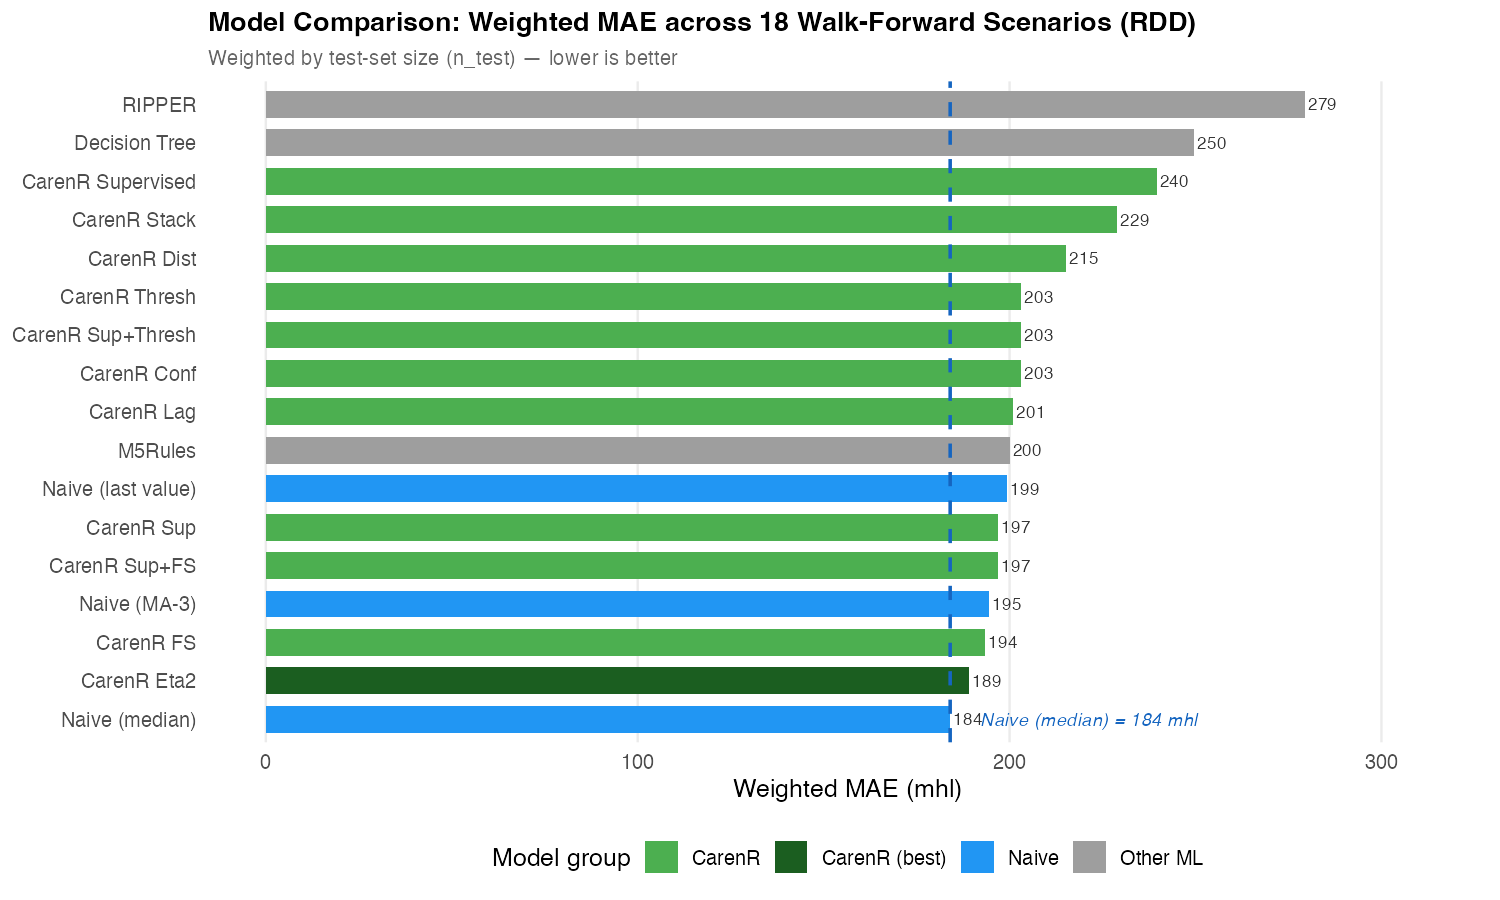
\includegraphics[width=0.92\textwidth]{figures/fig51_weighted_mae_rdd.png}
  \caption{Weighted MAE ranking across all 17 models for the Douro (RDD) region. Lower is better.}
  \label{fig:weighted_mae_rdd}
\end{figure}



\subsection{Vinho Verde (RVV)}\label{sub:vinho_verde_rvv}

For Vinho Verde, Naive\_Median again ranks first at 140\footnote{\textbf{[Defesa] P:} Nada bate a Naive\_Median --- o clima é irrelevante? \textbf{R:} Não; o sinal é real (LOESS retém 90--125\% no RDD) mas insuficiente face ao noise (CV cerca de 47\%). ``Afeta a produção'' e ``bate a baseline'' são claims diferentes.} mhl. The best CarenR variant is CarenR\_Dist\_Sup\_FS at 172 mhl, a gap of 31 mhl (22\%) relative to the naive baseline. CarenR\_Dist\_Eta2, the best RDD model, drops from rank 2 in RDD to rank 12 in RVV (226 mhl), a rank reversal of 10 positions. RIPPER reaches 508 mhl and Decision Tree 479 mhl.

\begin{table}[htbp]
  \centering
  \caption{RVV walk-forward results sorted by weighted MAE (mhl).}\label{tab:ch5a_2}
  \small
  \begin{adjustbox}{max width=\textwidth}
    \begin{tabularx}{\textwidth}{l|p{4.5cm}|l|l|X}
  \toprule
  Rank & Model & Weighted MAE (mhl) & Rank in RDD & Rank shift vs RDD \\
  \midrule
  1 & Naive\_Median & 140.4 & 1 & 0 \\
  2 & Naive & 143.8 & 7 & +5 \\
  3 & Naive\_MA & 170.5 & 4 & +1 \\
  4 & CarenR\_Dist\_Sup\_FS & 171.6 & 5 & +1 \\
  5 & CarenR\_Dist\_Sup\_Thresh & 171.6 & 11 & +6 \\
  6 & CarenR\_Dist\_Conf & 171.6 & 10 & +4 \\
  7 & CarenR\_Dist\_Sup & 185.2 & 6 & -1 \\
  8 & CarenR\_Dist\_Stack & 196.2 & 14 & +6 \\
  9 & CarenR\_Dist\_Thresh & 209.4 & 12 & +3 \\
  10 & CarenR\_Dist\_FS & 222.4 & 3 & -7 \\
  11 & CarenR\_Dist\_Lag & 225.0 & 9 & -2 \\
  12 & CarenR\_Dist\_Eta2 & 225.7 & 2 & -10 \\
  13 & M5Rules & 267.5 & 8 & -5 \\
  14 & CarenR\_Dist & 274.6 & 13 & -1 \\
  15 & CarenR\_Supervised & 347.3 & 15 & 0 \\
  16 & DT & 479.3 & 16 & 0 \\
  17 & Ripper & 508.2 & 17 & 0 \\
  \bottomrule
\end{tabularx}
  \end{adjustbox}

\end{table}


\begin{figure}[htbp]
  \centering
  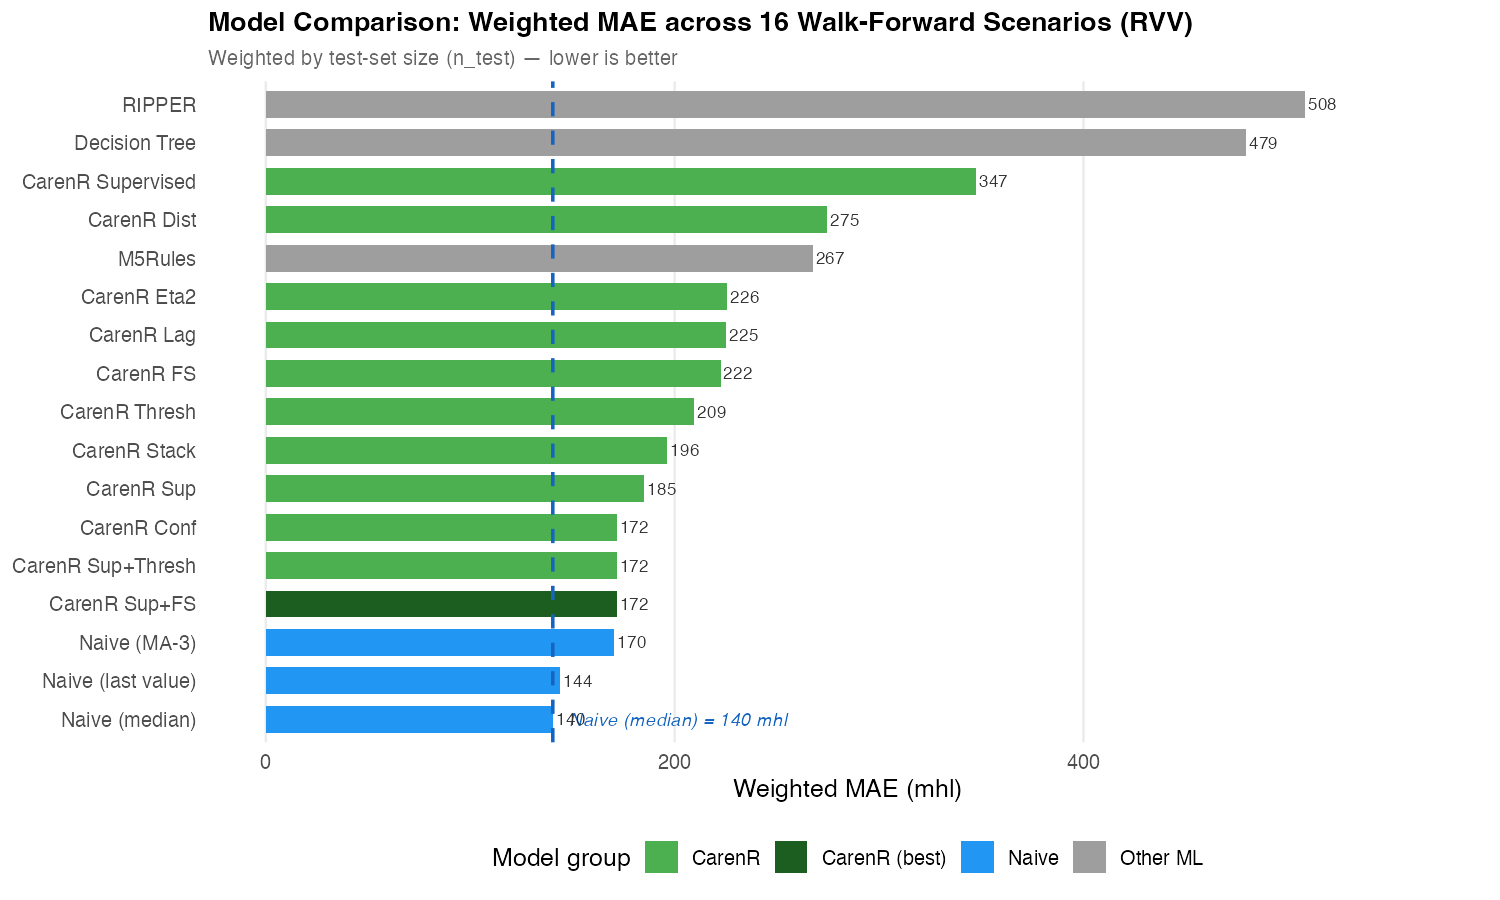
\includegraphics[width=0.92\textwidth]{figures/fig52_weighted_mae_rvv.png}
  \caption{Weighted MAE ranking across all 17 models for the Vinho Verde (RVV) region.}
  \label{fig:weighted_mae_rvv}
\end{figure}



\section{Era Composition and Per-Scenario Analysis (RDD)}\label{sec:era_composition_and_perscenario}

To investigate whether the aggregate weighted MAE obscures important structure, the per-scenario MAE for CarenR\_Dist\_Eta2 was examined alongside the proportion of post-1990 observations in each training fold. This analysis was conducted after observing the aggregate results; it is therefore exploratory, and all conclusions drawn from it should be read as hypothesis-generating rather than confirmatory.

\begin{table}[htbp]
  \centering
  \caption{Per-scenario \texttt{CarenR\_Dist\_Eta2} vs \texttt{Naive\_Median} for RDD.}\label{tab:ch5a_3}
  \small
  \begin{adjustbox}{max width=\textwidth}
    \begin{tabularx}{\textwidth}{p{3cm}|p{1.7cm}|p{1.7cm}|p{1.9cm}|p{2.6cm}|X}
  \toprule
  Phase & Scenarios & Post-1990 share & Test window & CarenR vs Naive\_Median & CarenR wins? \\
  \midrule
  Early, era-confounded & 1--9 & 20--28\% & 10--18 years & +5 to +28 mhl & No (7/9 losses) \\
  Balanced era & 10--14 & 29--32\% & 5--9 years & -17 to -32 mhl & Yes (5/5 wins) \\
  Late, tiny test sets & 15--18 & 33--35\% & 1--4 years & Noisy & Unreliable \\
  \bottomrule
\end{tabularx}
  \end{adjustbox}

\end{table}


\begin{figure}[htbp]
  \centering
  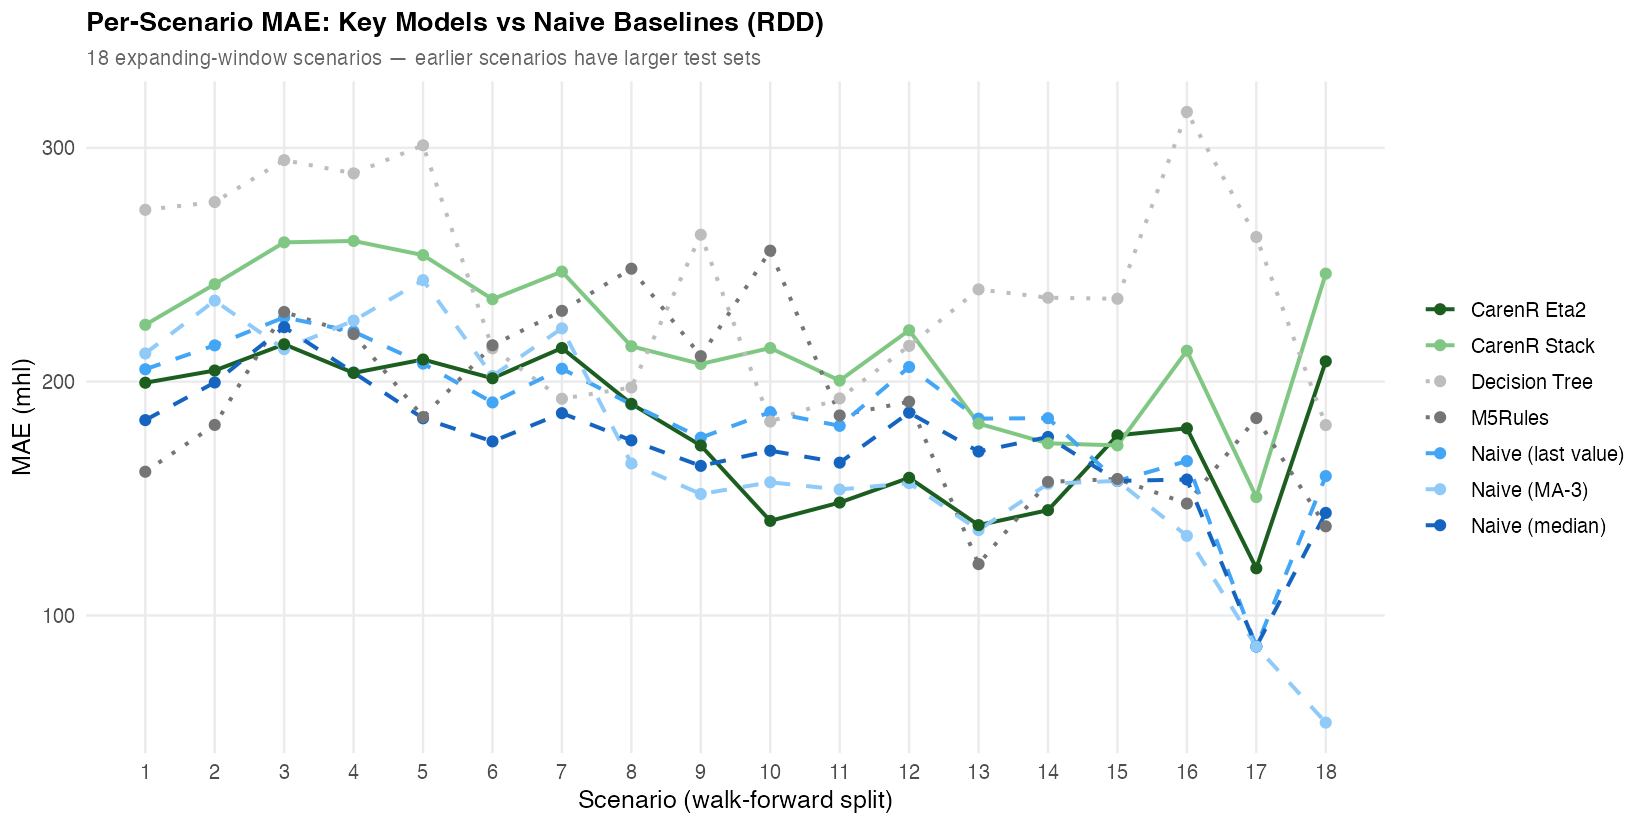
\includegraphics[width=0.92\textwidth]{figures/fig53_per_scenario_rdd.png}
  \caption{Per-scenario MAE for \texttt{CarenR\_Dist\_Eta2} vs \texttt{Naive\_Median} (RDD).}
  \label{fig:per_scenario_rdd}
\end{figure}


In scenarios 10--14, once the post-1990 share of training data reaches approximately 29\%, CarenR\_Dist\_Eta2 beats the Naive\_Median in every scenario by margins of 17--32 mhl. In early scenarios (post-1990 share 20--28\%), CarenR loses in 7 of 9 scenarios. The aggregate weighted MAE still places CarenR behind the baseline (189 vs 184 mhl) because early scenarios have the largest test sets (18 years in Scenario 1 vs 5 years in Scenario 14) and therefore dominate the weighted aggregate.


\section{Era Composition and Per-Scenario Analysis (RVV)}\label{sec:era_composition_and_perscenario_rvv}

The era-composition analysis was applied to RVV to test whether a similar improvement pattern appears. The result is unambiguous: across all 16 RVV scenarios, CarenR achieves zero wins against the Naive\_Median. As more post-1990 data enters the training set, CarenR's performance in RVV worsens rather than improves, the opposite direction from RDD.

\begin{table}[htbp]
  \centering
  \caption{RVV scenario outcomes for \texttt{CarenR\_Dist\_Sup\_FS} vs \texttt{Naive\_Median}.}\label{tab:ch5a_4}
  \small
  \begin{adjustbox}{max width=\textwidth}
    \begin{tabularx}{\textwidth}{l|l|X}
  \toprule
  Outcome & Count & Interpretation \\
  \midrule
  Identical to Naive\_Median (fallback) & 7 / 16 & No rules fired: CarenR predicted training median \\
  Worse than Naive\_Median & 9 / 16 & Rules fired but hurt prediction, harmful rules applied \\
  Better than Naive\_Median & 0 / 16 & CarenR never beats the naive baseline in any scenario \\
  \bottomrule
\end{tabularx}
  \end{adjustbox}

\end{table}


\begin{figure}[htbp]
  \centering
  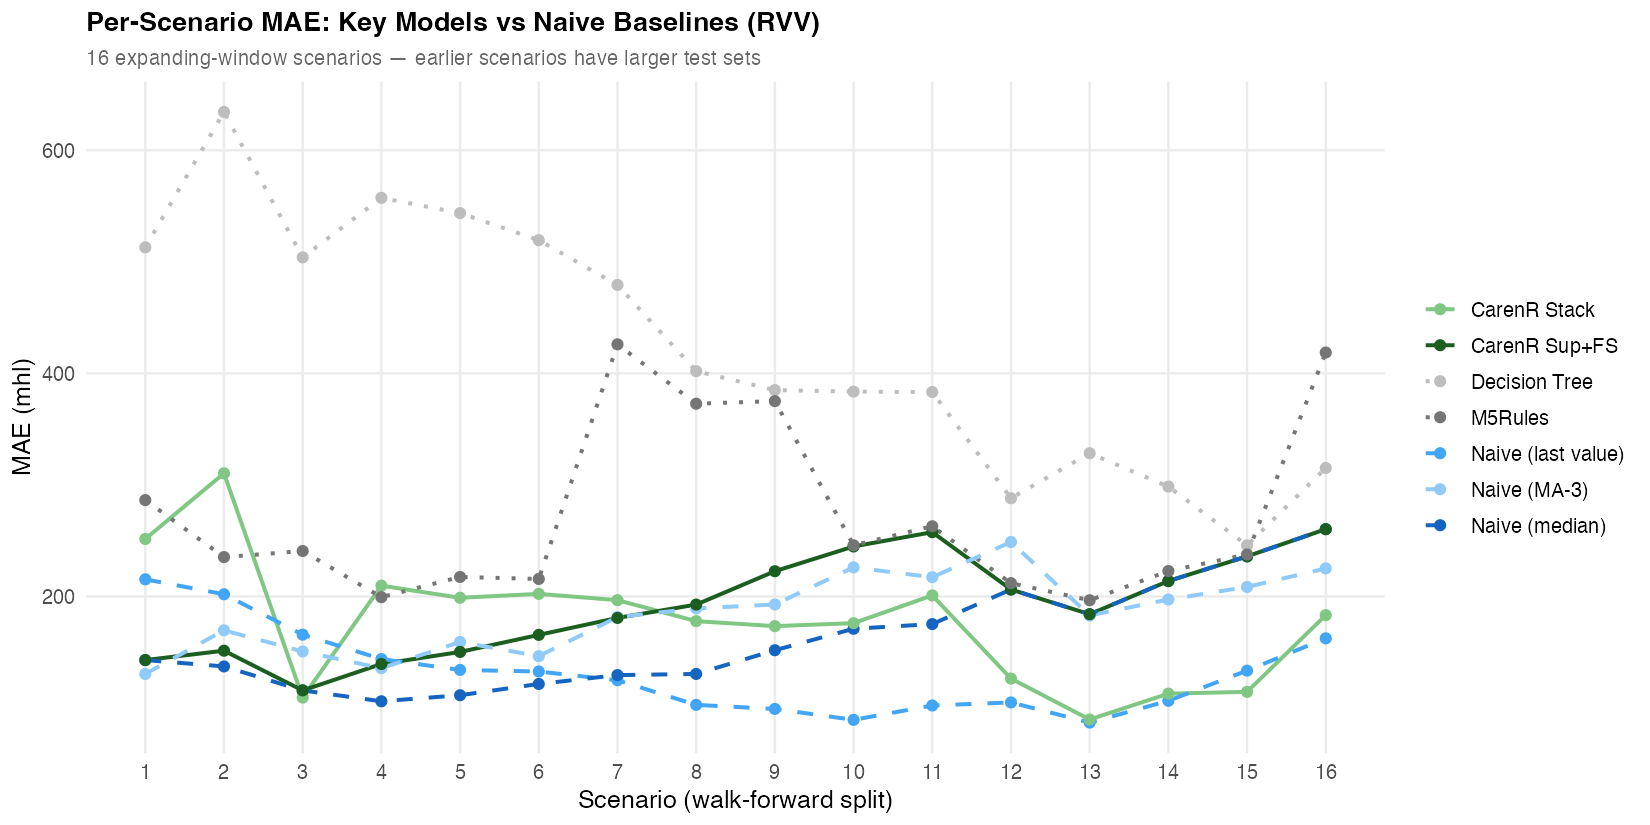
\includegraphics[width=0.92\textwidth]{figures/fig54_per_scenario_rvv.png}
  \caption{Per-scenario MAE for \texttt{CarenR\_Dist\_Sup\_FS} vs \texttt{Naive\_Median} (RVV).}
  \label{fig:per_scenario_rvv}
\end{figure}


\begin{table}[htbp]
  \centering
  \caption{RDD vs RVV summary comparison across key evaluation dimensions.}\label{tab:ch5a_5}
  \small
  \begin{adjustbox}{max width=\textwidth}
    \begin{tabularx}{\textwidth}{l|l|X}
  \toprule
  Dimension & RDD: Douro & RVV: Vinho Verde \\
  \midrule
  CarenR wins (any scenario) & 5 / 18 & 0 / 16 \\
  Effect of adding post-1990 data & Improves CarenR & Worsens CarenR \\
  Fallback to median (no rules) & Rare & 7 / 16 (44\%) \\
  Rules fire but hurt prediction & Some early scenarios & 9 / 16 (56\%) \\
  Best CarenR gap to Naive\_Median & +3\% (189 vs 184 mhl) & +22\% (172 vs 140 mhl) \\
  \bottomrule
\end{tabularx}
  \end{adjustbox}

\end{table}



\section{Statistical Tests}\label{sec:statistical_tests}

Three statistical tests were conducted. Tests are classified below as confirmatory (hypothesis specified before examining results) or exploratory (hypothesis identified after examining results). Uncorrected p-values are reported; no correction for multiple comparisons\footnote{\textbf{[Defesa] P:} 17 modelos sem multiple-comparison correction --- justifica os p-values. \textbf{R:} A primary comparison é única e pre-specified (best CarenR vs.\ Naive\_Median por região); a tabela de 17 é um descriptive ranking, não 17 tests. O headline é um nulo, logo a multiplicidade não fabrica um false positive. Reporto uncorrected e trato como exploratório.} was applied.

\textbf{Test 1 --- Overall RDD (confirmatory): }Wilcoxon signed-rank test, CarenR\_Dist\_Eta2 vs Naive\_Median\footnote{\textbf{[Defesa] P:} Porquê Wilcoxon signed-rank e não um paired t-test? \textbf{R:} Non-parametric; não assume normality das diferenças em small samples (18/16). Reporto exact p-values e sinalizo a baixa power.}, 18 scenarios. Result: W = 68, p = 0.468\footnote{\textbf{[Defesa] P:} Os 18 scenarios partilham anos de teste --- o Wilcoxon é válido? \textbf{R:} Estão positivamente correlacionados, o que torna o teste menos propenso a significância (consistente com o nulo p=0,468). Reporto os p-values como indicativos, não exatos.}. Not significant. CarenR does not significantly outperform or underperform the naive baseline in aggregate.

\textbf{Test 2 --- Era-balanced RDD scenarios 10--14\footnote{\textbf{[Defesa] P:} 5/5 wins com n=5 post-hoc --- data dredging? \textbf{R:} Sim, é post-hoc e exploratório e rotulo-o como tal. Gera uma hypothesis (pré-registar e testar em dados 2023+), não a confirma. Não defender como evidência.} (exploratory / post-hoc): }Binomial sign test on 5 scenarios where CarenR won in all 5. The scenarios were identified as era-balanced after observing that CarenR won in them, not pre-specified. Result: p = 0.031. Although this meets the $\alpha$ = 0.05 threshold, the post-hoc identification of the scenario window means this result must be treated as exploratory. It generates a testable hypothesis, that CarenR outperforms the naive baseline when post-1990 training share reaches ~29\%, but does not confirm it. Independent prospective validation on new data is required before treating this as a robust finding. This result is referred to throughout this thesis as a post-hoc exploratory finding.

\textbf{Test 3 --- RVV rule-firing scenarios (confirmatory): }Wilcoxon signed-rank test on the 9 RVV scenarios where CarenR fired rules (excluding 7 fallback scenarios). Result: W = 0, p = 0.004. Highly significant. When CarenR fires rules in Vinho Verde, those rules are significantly worse than the naive baseline. CarenR's rules actively harm predictive accuracy in RVV. This is a confirmatory negative result.

\begin{table}[htbp]
  \centering
  \caption{Statistical tests summary. The $p=0.031$ result is exploratory.}\label{tab:ch5a_6}
  \small
  \begin{adjustbox}{max width=\textwidth}
    \begin{tabularx}{\textwidth}{p{2.2cm}|p{3.8cm}|p{1.6cm}|p{1.2cm}|X}
  \toprule
  Test & Comparison & Statistic & p-value & Classification \\
  \midrule
  Wilcoxon (2-sided) & CarenR\_Dist\_Eta2 vs Naive\_Median, RDD, all 18 scenarios & W = 68 & 0.468 & Confirmatory, not significant \\
  Binomial sign test & CarenR wins 5/5 era-balanced scenarios (10--14), RDD & p(k$\geq$5, n=5) & 0.031 & POST-HOC / EXPLORATORY, requires prospective validation \\
  Wilcoxon (2-sided) & CarenR\_Dist\_Sup\_FS vs Naive\_Median, RVV, 9 rule-firing scenarios & W = 0 & 0.004 & Confirmatory, highly significant negative result \\
  \bottomrule
\end{tabularx}
  \end{adjustbox}

\end{table}



\section{Detrend Sensitivity Analysis (LOESS)}\label{sec:detrend_sensitivity_analysis_loess}

LOESS detrending (span = 0.40) reduces the Naive\_Median weighted MAE from 140 to ~90 mhl for RVV (-36\% improvement in Decision 1) but eliminates all CarenR rules (0 rules fire in all 16 scenarios). For RDD, LOESS worsens the baseline from 184 to 290 mhl (+58\%) because LOESS extrapolates a slope that the Douro's plateau-shaped trajectory does not follow. The LOESS results confirm that the choice of detrend method is region-specific and that improving Decision 1 comes at the direct cost of suppressing the signal required for Decision 2.

Figures~\ref{fig:detrend_rdd} and~\ref{fig:detrend_rvv} show the weighted MAE of all 17 models under both detrending methods for each region.

\begin{figure}[htbp]
  \centering
  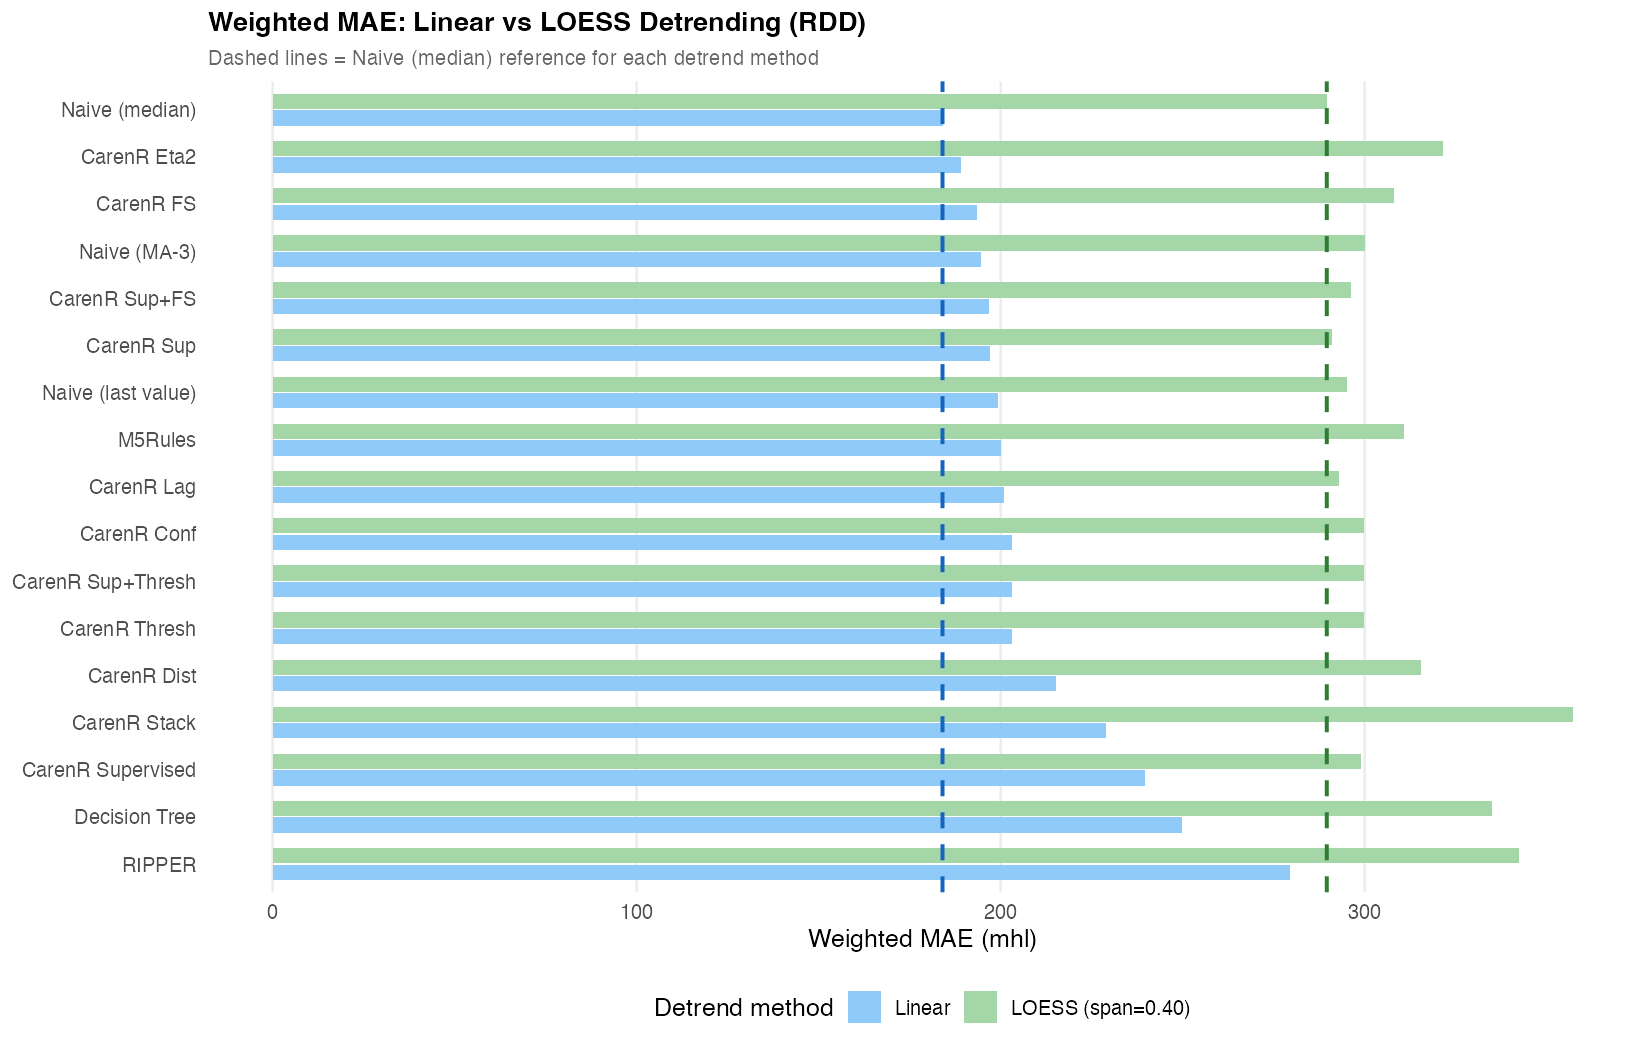
\includegraphics[width=0.85\textwidth]{figures/fig_detrend_rdd.png}
  \caption{Weighted MAE under linear vs LOESS detrending for all 17 models, Douro (RDD).}
  \label{fig:detrend_rdd}
\end{figure}

\begin{figure}[htbp]
  \centering
  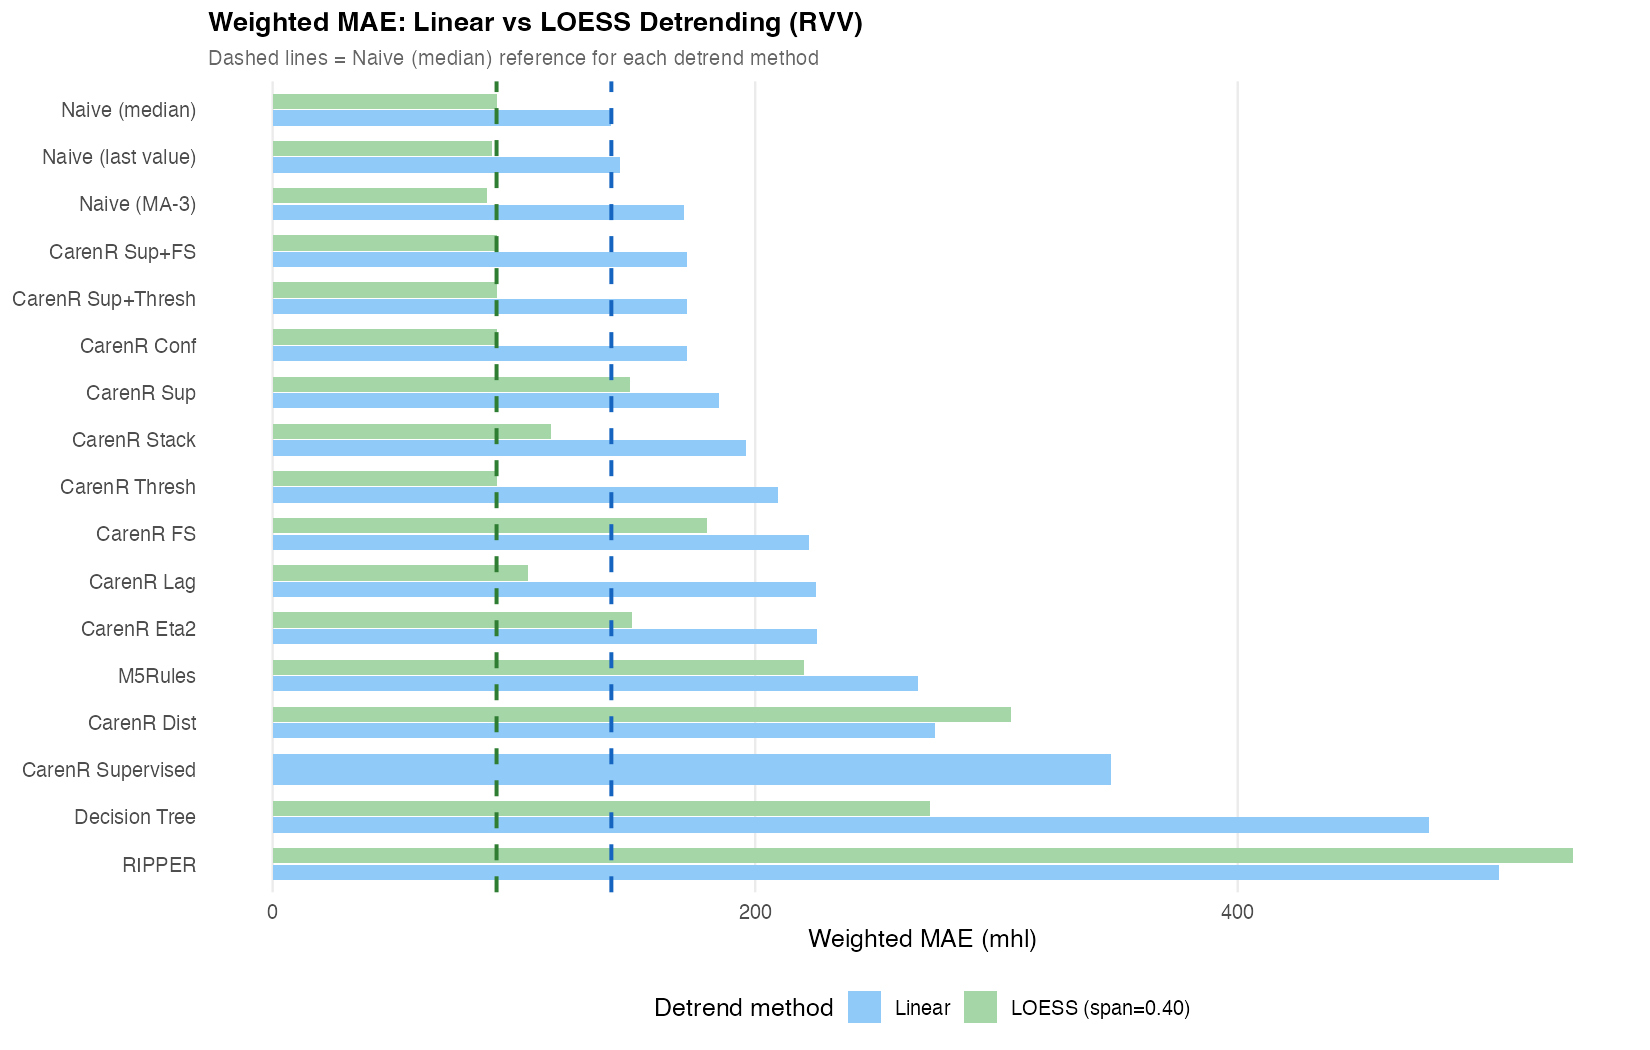
\includegraphics[width=0.85\textwidth]{figures/fig_detrend_rvv.png}
  \caption{Weighted MAE under linear vs LOESS detrending for all 17 models, Vinho Verde (RVV).}
  \label{fig:detrend_rvv}
\end{figure}


\begin{table}[htbp]
  \centering
  \caption{LOESS detrending sensitivity analysis.}\label{tab:ch5a_7}
  \small
  \begin{adjustbox}{max width=\textwidth}
    \begin{tabularx}{\textwidth}{l|p{3cm}|p{2.6cm}|p{2.2cm}|X}
  \toprule
  Region & Detrend & Naive\_Median wtd MAE & CarenR rules found & CarenR best wtd MAE \\
  \midrule
  RDD & Linear (primary) & 184 mhl & 48 & 189 mhl (Eta2) \\
  RDD & LOESS (sensitivity) & 290 mhl & N/A & --- \\
  RVV & Linear (primary) & 140 mhl & 20 & 172 mhl (Sup\_FS) \\
  RVV & LOESS (sensitivity) & ~90 mhl & 0 (suppressed) & Falls back to median \\
  \bottomrule
\end{tabularx}
  \end{adjustbox}

\end{table}



\section{Negative Results: Supervised Discretisation}\label{sec:negative_results_supervised_discretisation}

CarenR\_Supervised, which uses supervised feature discretisation --- deriving bin cut-points by maximising residual separation within each training fold rather than relying on equal-frequency quantiles --- was the worst-performing CarenR variant in both regions (rank 15; RDD 240 mhl, RVV 347 mhl). It discovers 46--146 rules per scenario, substantially more than the unsupervised variants, but the rules overfit the training fold because the bin boundaries are optimised on the same data used to assess rule quality. This is a form of target leakage in the feature engineering step. The result is consistent across both regions, confirming that per-fold supervised discretisation degrades out-of-sample performance regardless of climate regime.


\section{Summary: Predictive Validation Assessment (Goal 2)}\label{sec:summary_of_goal_2}

No model beats Naive\_Median in aggregate in either region. The best CarenR variant falls 3\footnote{\textbf{[Defesa] P:} Escolheste a best de 11 variantes depois de ver os resultados --- selection bias. \textbf{R:} Sim, e isso reforça a conclusão: mesmo a best variant post-hoc não bate a Naive\_Median. Reporto as 11. A retrospective selection só importaria se eu reivindicasse vitória.}\% behind in RDD (Wilcoxon p = 0.468) and 22\% behind in RVV. The 22\% gap in RVV is accompanied by a confirmatory finding that CarenR's rules actively harm prediction when they fire (p = 0.004). A post-hoc exploratory analysis (p = 0.031, n = 5 scenarios) suggests CarenR may be competitive in the Douro when training data is era-balanced, but this observation requires independent validation before it can be treated as a robust finding. Goal 2 is assessed as not achieved in aggregate, with a conditional observation in the RDD era-balanced window that motivates future prospective investigation.


% ===== CONTINUATION =====


\section{Per-Scenario MAE: Douro (RDD)}\label{sec:perscenario_mae_douro_rdd}

Table~\ref{tab:ch5b_1} presents the complete per-scenario MAE values for Naive\_Median and CarenR\_Dist\_Eta2 across all 18 RDD scenarios. The gap column (positive = CarenR worse, negative = CarenR better) reveals the era-composition pattern described in Section~\ref{sec:era_composition_and_perscenario}. Scenarios 10--14, highlighted in green, are the five consecutive era-balanced scenarios where CarenR outperforms the naive baseline. The training period for each scenario is 1934 through the year indicated; the test period begins the year immediately following and extends to 2022.

\begin{table}[htbp]
  \centering
  \caption{Per-scenario MAE for \texttt{Naive\_Median} and \texttt{CarenR\_Dist\_Eta2}: 18 RDD scenarios.}\label{tab:ch5b_1}
  \small
  \begin{adjustbox}{max width=\textwidth}
    \begin{tabularx}{\textwidth}{p{0.7cm}|p{1.6cm}|p{1.6cm}|p{1.5cm}|p{1.5cm}|p{1.6cm}|X}
  \toprule
  Scen. & Train period & Test period & Naive\_Median
MAE (mhl) & CarenR\_Eta2
MAE (mhl) & Gap
(+ = CarenR worse) & Era phase \\
  \midrule
  1 & 1934--2004 & 2005--2022 & 183.5 & 199.5 & +16.0 & Early, era-confounded \\
  2 & 1934--2005 & 2006--2022 & 199.7 & 204.8 & +5.1 & Early, era-confounded \\
  3 & 1934--2006 & 2007--2022 & 223.3 & 216.0 & -7.3 & Early, marginal CarenR win \\
  4 & 1934--2007 & 2008--2022 & 203.9 & 203.7 & -0.2 & Early, near-tie \\
  5 & 1934--2008 & 2009--2022 & 184.3 & 209.5 & +25.1 & Early, era-confounded \\
  6 & 1934--2009 & 2010--2022 & 174.4 & 201.4 & +27.0 & Early, era-confounded \\
  7 & 1934--2010 & 2011--2022 & 186.5 & 214.4 & +27.9 & Early, era-confounded \\
  8 & 1934--2011 & 2012--2022 & 174.9 & 190.5 & +15.6 & Early, era-confounded \\
  9 & 1934--2012 & 2013--2022 & 164.0 & 172.7 & +8.7 & Early, era-confounded \\
  10 & 1934--2013 & 2014--2022 & 170.5 & 140.5 & -30.0 & Balanced era $\star$ CarenR wins \\
  11 & 1934--2014 & 2015--2022 & 165.4 & 148.3 & -17.1 & Balanced era $\star$ CarenR wins \\
  12 & 1934--2015 & 2016--2022 & 186.7 & 158.9 & -27.9 & Balanced era $\star$ CarenR wins \\
  13 & 1934--2016 & 2017--2022 & 170.1 & 138.6 & -31.5 & Balanced era $\star$ CarenR wins \\
  14 & 1934--2017 & 2018--2022 & 176.3 & 145.0 & -31.3 & Balanced era $\star$ CarenR wins \\
  15 & 1934--2018 & 2019--2022 & 157.6 & 177.0 & +19.5 & Late, small test sets \\
  16 & 1934--2019 & 2020--2022 & 158.1 & 180.1 & +21.9 & Late, small test sets \\
  17 & 1934--2020 & 2021--2022 & 86.7 & 120.2 & +33.4 & Late: 2 yr test, noisy \\
  18 & 1934--2021 & 2022 & 143.9 & 208.7 & +64.8 & Late: 1 yr test, noisy \\
  \bottomrule
\end{tabularx}
  \end{adjustbox}

\end{table}


\begin{figure}[htbp]
  \centering
  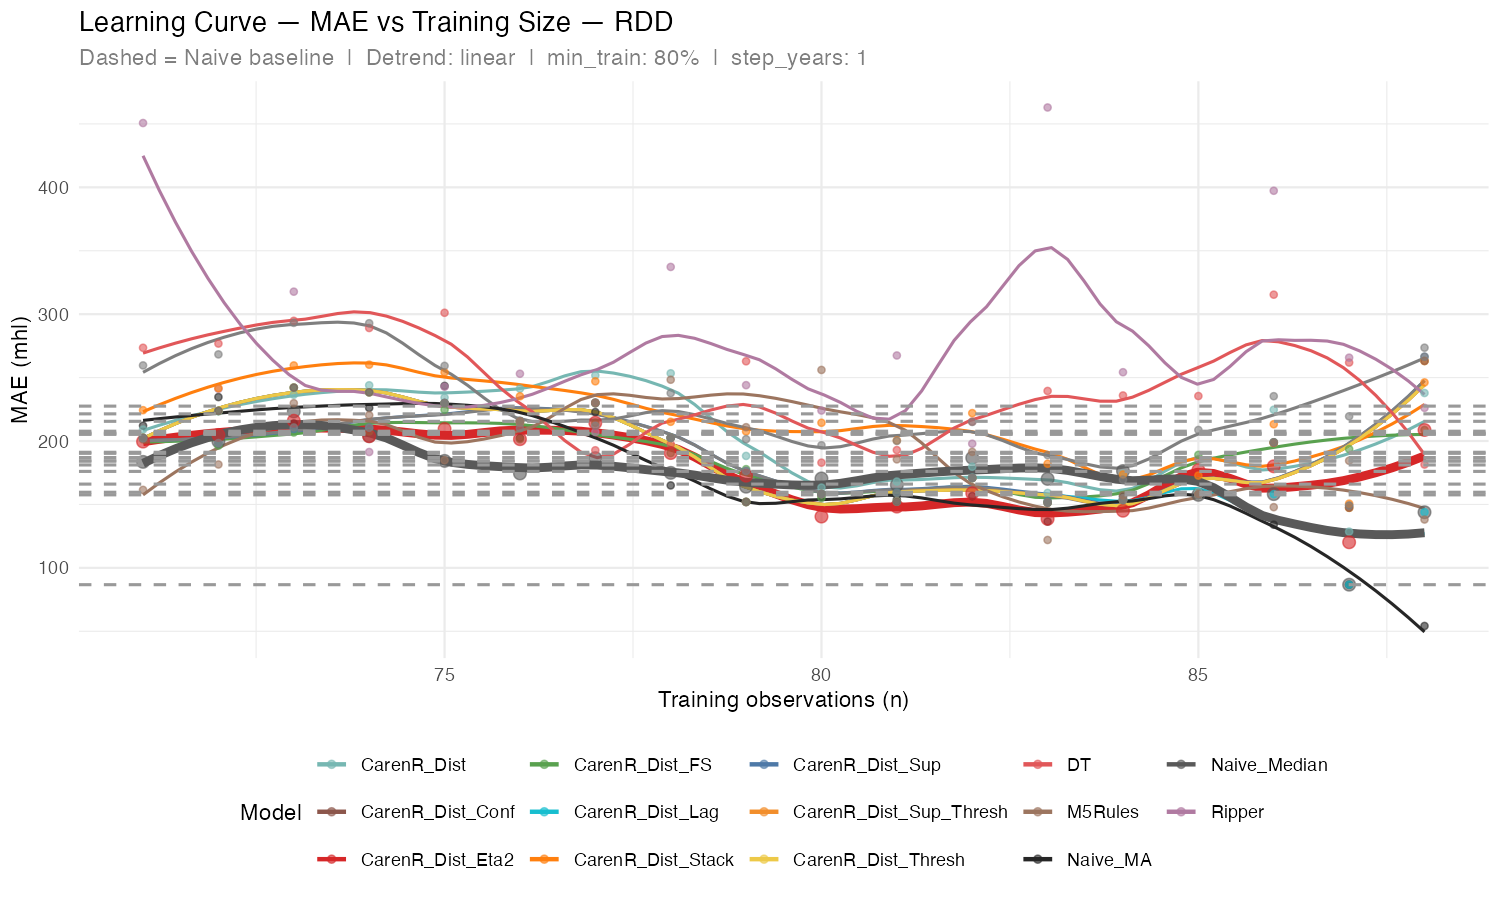
\includegraphics[width=0.92\textwidth]{figures/fig55_learning_curve_rdd.png}
  \caption{MAE learning curve for all 17 models across 18 RDD scenarios. LOESS smoothing applied.}
  \label{fig:learning_curve_rdd}
\end{figure}


Several observations from Table~\ref{tab:ch5b_1} are worth highlighting beyond the era-composition pattern already discussed in Section~\ref{sec:era_composition_and_perscenario}.

\textbf{Scenarios 3 and 4 (marginal CarenR wins, -7.3 and -0.2 mhl): }These two early scenarios show CarenR marginally matching or beating the naive baseline, despite low post-1990 training share (~22\%). They do not represent reliable era-balanced wins; their margins are near-zero and not consistent across the broader early window.

\textbf{Scenarios 17 and 18 (large positive gaps, +33 and +65 mhl): }Scenario 17 tests two years (2021--2022) and Scenario 18 tests a single year (2022). With very small test sets, the scenario MAE reflects only one or two observations, so large gaps may reflect anomalous years rather than systematic model failure. These late scenarios were therefore excluded from the era-balanced binomial analysis (Section~\ref{sec:statistical_tests}).

\textbf{Scenario Naive\_Median MAE range (86.7--223.3 mhl): }The variation in Naive\_Median MAE across scenarios reflects the inherent year-to-year production variability of the test year in each case. When the test year happens to be close to the trend (Scenario 17: 2021 was near-trend), Naive\_Median performs very well. When the test year is a strong outlier (Scenario 3: 2007 was above-trend in Douro), Naive\_Median has a high error regardless of what any model does. This variability confirms the importance of using weighted aggregate metrics rather than relying on any single scenario.


\section{Per-Scenario MAE: Vinho Verde (RVV)}\label{sec:perscenario_mae_vinho_verde}

Table~\ref{tab:ch5b_2} presents the equivalent per-scenario analysis for RVV, comparing Naive\_Median against CarenR\_Dist\_Sup\_FS (the best RVV CarenR variant). The ``outcome'' column indicates whether CarenR fell back to the median (identical prediction, zero gap) or fired rules that hurt prediction (positive gap).

\begin{table}[htbp]
  \centering
  \caption{Per-scenario MAE for \texttt{Naive\_Median} and \texttt{CarenR\_Dist\_Sup\_FS}: 16 RVV scenarios.}\label{tab:ch5b_2}
  \small
  \begin{adjustbox}{max width=\textwidth}
    \begin{tabularx}{\textwidth}{p{0.7cm}|p{1.6cm}|p{1.6cm}|p{1.5cm}|p{1.5cm}|p{1.6cm}|X}
  \toprule
  Scen. & Train period & Test period & Naive\_Median
MAE (mhl) & CarenR\_Sup\_FS
MAE (mhl) & Gap
(+ = CarenR worse) & Outcome \\
  \midrule
  1 & 1942--2005 & 2006--2021 & 143.0 & 143.0 & +0.0 & FALLBACK, no rules fired \\
  2 & 1942--2006 & 2007--2021 & 137.3 & 151.4 & +14.1 & HARMFUL, rules fired, hurt prediction \\
  3 & 1942--2007 & 2008--2021 & 115.7 & 115.7 & +0.0 & FALLBACK, no rules fired \\
  4 & 1942--2008 & 2009--2021 & 106.0 & 139.4 & +33.4 & HARMFUL, rules fired, hurt prediction \\
  5 & 1942--2009 & 2010--2021 & 111.4 & 150.2 & +38.8 & HARMFUL, rules fired, hurt prediction \\
  6 & 1942--2010 & 2011--2021 & 121.5 & 165.5 & +44.0 & HARMFUL, rules fired, hurt prediction \\
  7 & 1942--2011 & 2012--2021 & 129.5 & 180.8 & +51.3 & HARMFUL, rules fired, hurt prediction \\
  8 & 1942--2012 & 2013--2021 & 130.5 & 192.7 & +62.2 & HARMFUL, rules fired, hurt prediction \\
  9 & 1942--2013 & 2014--2021 & 151.8 & 222.6 & +70.8 & HARMFUL, rules fired, worst gap \\
  10 & 1942--2014 & 2015--2021 & 171.0 & 244.8 & +73.8 & HARMFUL, rules fired, worst gap \\
  11 & 1942--2015 & 2016--2021 & 175.2 & 257.6 & +82.4 & HARMFUL, rules fired, largest gap \\
  12 & 1942--2016 & 2017--2021 & 206.2 & 206.2 & +0.0 & FALLBACK, no rules fired \\
  13 & 1942--2017 & 2018--2021 & 184.0 & 184.0 & +0.0 & FALLBACK, no rules fired \\
  14 & 1942--2018 & 2019--2021 & 213.8 & 213.8 & +0.0 & FALLBACK, no rules fired \\
  15 & 1942--2019 & 2020--2021 & 235.9 & 235.9 & +0.0 & FALLBACK, no rules fired \\
  16 & 1942--2020 & 2021 & 260.3 & 260.3 & +0.0 & FALLBACK, no rules fired \\
  \bottomrule
\end{tabularx}
  \end{adjustbox}

\end{table}


\begin{figure}[htbp]
  \centering
  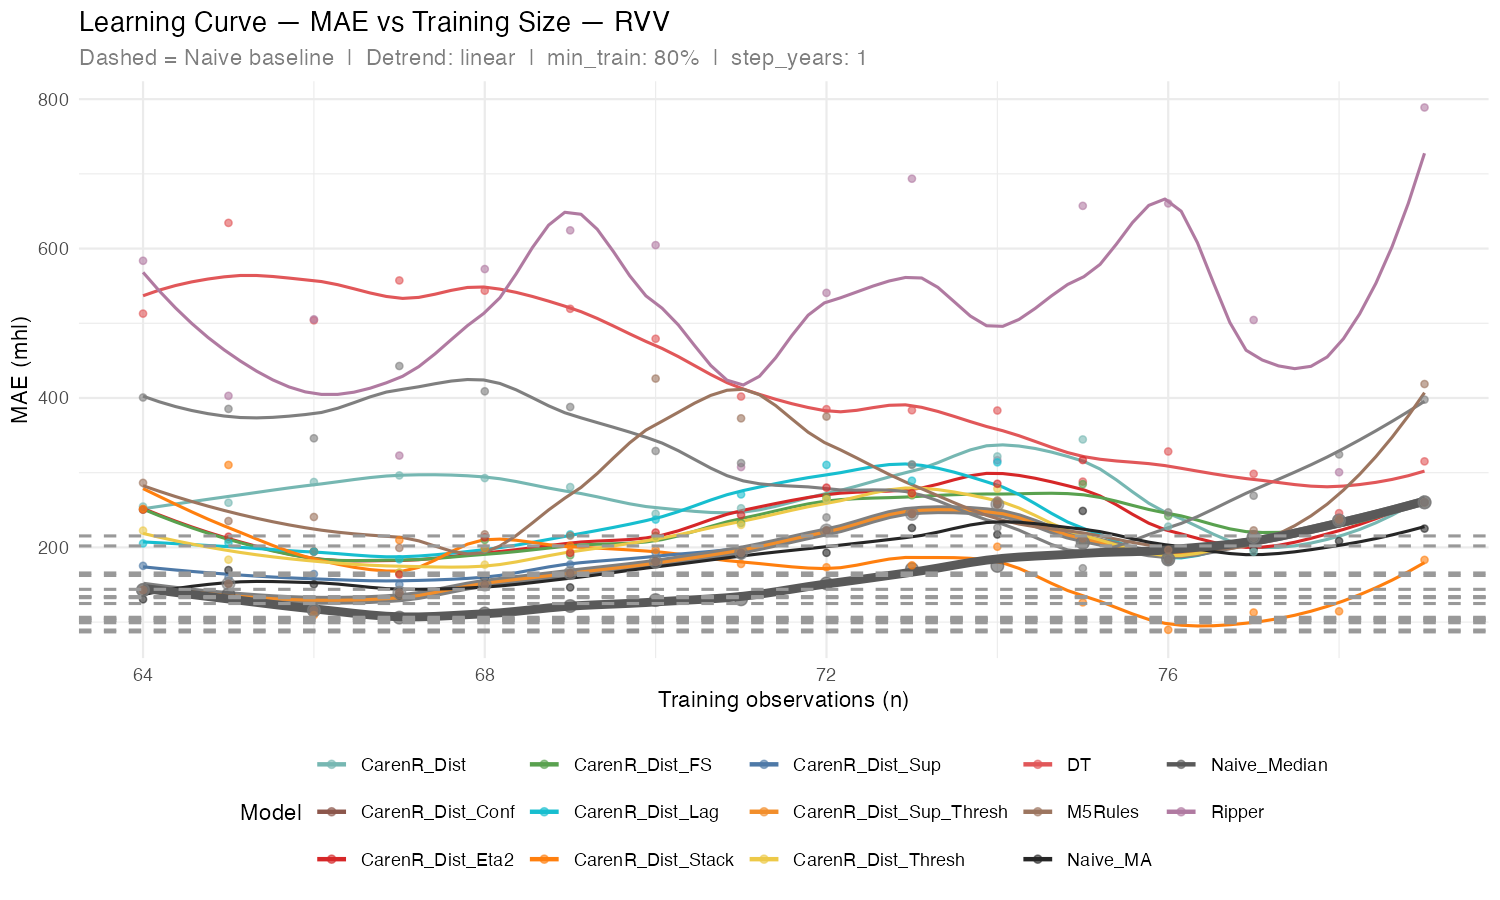
\includegraphics[width=0.92\textwidth]{figures/fig56_learning_curve_rvv.png}
  \caption{MAE learning curve for all 17 models across 16 RVV scenarios. LOESS smoothing applied.}
  \label{fig:learning_curve_rvv}
\end{figure}


The RVV per-scenario table reveals important structure that the aggregate weighted MAE figure of 172 mhl obscures.

\textbf{The degradation trajectory (Scenarios 4--11): }The gap between CarenR and the naive baseline grows monotonically from +33 mhl (Scenario 4) to +82 mhl (Scenario 11). This is the clearest evidence of the era-composition deterioration described in Section~\ref{sec:era_composition_and_perscenario_rvv}: as the training set includes more post-1990 observations (with substantially lower production than the historical average), the rules CarenR discovers become increasingly calibrated to the modern low-production era. When those rules are applied to test years that are also in the modern era, they fire conditions that, by coincidence, match the training set's era characteristics rather than genuine inter-annual climate signals, and predict in the wrong direction.

\textbf{The fallback pattern (Scenarios 1, 3, 12--16): }Seven of 16 scenarios show a zero gap, CarenR fired no rules and fell back to the training median. This is not a failure in the same sense as the harmful-rules scenarios: it means no CarenR rule achieved sufficient support to fire, and the prediction framework fell back to the training median as the safe default. The fallback scenarios are concentrated in early scenarios (1, 3) and late scenarios (12--16). The late fallback pattern is interesting: in scenarios 12--16, the training set is very era-balanced (all modern era), but CarenR apparently finds no applicable rules. This suggests that with a homogeneous modern-era training set, the wine production signal becomes too noisy for any subgroup to achieve both KS significance and $\geq$20\% support, confirming that the era structure is what created the spurious rules in the first place.

\textbf{Weighted MAE decomposition: }The weighted aggregate of 172 mhl is dominated by the 9 harmful scenarios (weighted by test-set sizes of 20--80 years in early scenarios). The 7 fallback scenarios contribute 0 mhl to the gap. This means the 22\% gap between CarenR and Naive\_Median in RVV is entirely attributable to the harmful-rules scenarios, not to the fallback scenarios. The Wilcoxon test on harmful-rules scenarios (p = 0.004, Section~\ref{sec:statistical_tests}) correctly identifies these as the source of the problem.


% ===== CONTINUATION =====


\section{Feature Selector Comparison: Why Eta2 Wins in RDD and Sup\_FS in RVV}\label{sec:feature_selector_comparison_why}

The 11 CarenR variants evaluated in this study differ primarily in their feature selection strategy, the step that reduces the 59-feature input space before CarenR searches for rules. This section analyses why different selection strategies produce different outcomes across the two regions, and what that tells us about the underlying agroclimatic signal.

\begin{table}[htbp]
  \centering
  \caption{CarenR variant sensitivity analysis by feature selection strategy.}\label{tab:ch5c_1}
  \small
  \begin{adjustbox}{max width=\textwidth}
    \begin{tabularx}{\textwidth}{p{3.2cm}|p{3.6cm}|p{1.7cm}|p{1.5cm}|p{1.7cm}|X}
  \toprule
  Variant & Selection method & RDD rank
(among CarenR) & RDD wtd MAE & RVV rank
(among CarenR) & RVV wtd MAE \\
  \midrule
  CarenR\_Dist\_Eta2 & $\eta$$^2$ ANOVA effect size & 1st & 189.2 & 9th & 225.7 \\
  CarenR\_Dist\_FS & Pearson |r|, top-N & 2nd & 193.5 & 7th & 222.4 \\
  CarenR\_Dist\_Sup\_FS & Pearson |r| + support $\geq$20\% & 3rd & 196.9 & 1st & 171.6 \\
  CarenR\_Dist\_Sup & Pearson + support filter & 4th & 197.0 & 4th & 185.2 \\
  CarenR\_Dist\_Lag & ACF-based lag features & 5th & 200.9 & 8th & 225.0 \\
  CarenR\_Dist\_Conf & Confidence-weighted rules & 6th & 203.1 & 3rd & 171.6 \\
  CarenR\_Dist\_Sup\_Thresh & Pearson + support + threshold & 7th & 203.1 & 2nd & 171.6 \\
  CarenR\_Dist\_Thresh & Pearson hard threshold |r|$\geq$0.30 & 8th & 203.1 & 6th & 209.4 \\
  CarenR\_Dist & No selection (all features) & 9th & 215.3 & 10th & 274.6 \\
  CarenR\_Dist\_Stack & Two-stage stacking & 10th & 229.0 & 5th & 196.2 \\
  CarenR\_Supervised & Per-fold supervised bins & 11th & 239.5 & 11th & 347.3 \\
  \bottomrule
\end{tabularx}
  \end{adjustbox}

\end{table}


The rank reversals are striking: CarenR\_Dist\_Eta2 ranks 1st in RDD but 9th in RVV; CarenR\_Dist\_Sup\_FS ranks 3rd in RDD and 1st in RVV. Understanding why requires examining what each selector does and why that matters differently in each region.

\textbf{Why $\eta$$^2$ wins in RDD. }The $\eta$$^2$ (eta-squared) selector measures the association between each discretised feature and the discretised response using an ANOVA effect size; it detects whether the production distribution differs meaningfully across the four quartile bins of each feature. In the Douro, where genuine climate signal exists and CarenR actually fires rules in several scenarios, the quality of the feature selection matters: $\eta$$^2$ identifies the specific variables (harvest soil water, post-flowering wet days) whose distributional relationship with production is strongest within the training period. This results in rules that fire on genuinely informative conditions and improve prediction in the era-balanced scenarios. In Vinho Verde, where CarenR falls back to the median in most scenarios (rules do not fire, or fire harmfully), the quality of the feature selection is largely irrelevant, the prediction is dominated by the fallback mechanism regardless of which 10--15 features were retained. The $\eta$$^2$ variant's aggressive selection produces slightly harmful rules in the few RVV scenarios where it does fire, explaining its poor RVV rank.

\textbf{Why Sup\_FS wins in RVV. }CarenR\_Dist\_Sup\_FS applies a support filter on top of Pearson correlation selection: it retains only features where each bin contains at least 20\% of the training observations, ensuring that the feature's relationship with production is robust across the entire distribution rather than driven by a handful of extreme years. In Vinho Verde, where the dominant ``below-trend'' signal arises from a combination of multiple co-occurring conditions (soil water + heat stress + LAI), aggressive selection tends to produce overfit rules that fire on era-specific patterns rather than genuine climate signals. The conservative Sup\_FS selection retains only the most broadly applicable features, which produces rules that either fire correctly on obvious patterns or, most importantly, recognise that no confident rule applies and fall back to the median. The fallback behaviour is the key: in 7 of 16 RVV scenarios, Sup\_FS correctly predicts the median (zero gap vs Naive\_Median), whereas a more aggressive selector would fire a spurious rule and accumulate error.

The practical implication is clear: in regimes with strong and consistent climate signal (RDD), aggressive feature selection that identifies the most discriminating features improves prediction. In regimes with weaker or more era-contaminated signal (RVV), conservative selection that preserves the fallback mechanism is preferable. The optimal strategy is therefore problem-specific, which argues for the kind of structured sensitivity analysis, evaluating all 11 variants, that this thesis undertakes, rather than committing to a single variant a priori.


\section{What Happened in the Era-Balanced Winning Years?}\label{sec:what_happened_in_the}

The five scenarios where CarenR\_Dist\_Eta2 beats the naive baseline in RDD correspond to test-start years 2014--2018 (each test period extends to 2022). Understanding what made these years predictable from climate rules, and why CarenR succeeded where it fails in other years, provides important context for the post-hoc finding (p = 0.031).

In each of these five years, CarenR fired rules based on the top RDD signals, dry post-flowering conditions and moderate soil water stress at harvest, and its predicted above-trend residual was closer to the actual production than the training median. The training sets for scenarios 10--14 (covering 1934 through 2013--2017) had reached approximately 29--32\% post-1990 representation, meaning the discovered rules were calibrated on a training distribution that meaningfully included the modern (post-1990) production era rather than being dominated by the high-production pre-1976 era.

Agronomically, 2014--2018 were years characterised by the Douro's increasingly hot, dry summers, a pattern that has intensified under recent climate trends. The dry post-flowering and moderate pre-harvest soil water conditions that define the top CarenR rules were clearly present in multiple years of this window, creating genuine rule-fireable conditions that translated to above-trend production. The fact that CarenR could detect and predict this correctly, rather than falling back to the median, is precisely what the distributional rule framework is designed to achieve: identifying years where the climate signal is strong enough to be actionable.

The reason CarenR then fails again in scenarios 15--18 (test years 2019--2022) is equally informative. The 2019--2022 window was characterised by unusual year-to-year variability driven by the combined effects of climate extremes (severe drought years interspersed with unusually wet seasons). The rules learned from 1934--2018 training data were calibrated to the historical distributional structure, which was disrupted by the post-2018 volatility. This is a reminder that distributional rules are inherently backward-looking: they identify patterns from historical data, and their predictive value diminishes when the future departs from the historical distributional structure.


\section{The Fallback Mechanism: When CarenR Says ``I Don't Know''}\label{sec:the_fallback_mechanism_when}

A distinctive and underappreciated feature of the CarenR prediction framework is its explicit fallback mechanism: when no rule fires for a given test year, the model predicts the training median residual, the same prediction as the Naive\_Median baseline. This produces a zero gap between CarenR and Naive\_Median in those scenarios.

This behaviour is not a failure; it is the model correctly communicating uncertainty. A CarenR fallback is semantically equivalent to saying: ``the climate conditions of this test year do not match any of the patterns I learned from historical data with sufficient confidence. My best prediction is therefore the training median --- equivalent to the Naive\_Median baseline.'' This is a principled, conservative position that avoids compounding error by applying a rule that may not be appropriate.

The contrast with RIPPER is instructive. RIPPER always assigns a class; it has a default rule that catches all unmatched observations, and it will always produce a prediction. This means RIPPER never explicitly signals uncertainty; every test year gets a confident class assignment regardless of how well it matches the training patterns. The result is that RIPPER's errors in difficult years are often larger than CarenR's, because CarenR defaults to the safe median while RIPPER applies its default (most-common-class) rule.

\begin{table}[htbp]
  \centering
  \caption{The three possible outcomes of CarenR prediction and their interpretation.}\label{tab:ch5c_2}
  \small
  \begin{adjustbox}{max width=\textwidth}
    \begin{tabularx}{\textwidth}{p{2.4cm}|p{2.8cm}|p{2.2cm}|p{2.0cm}|X}
  \toprule
  Scenario type & CarenR behaviour & Prediction & Gap vs baseline & Interpretation \\
  \midrule
  Rules fire, correct direction & Applies matching rule(s) & Weighted rule mean & Negative (CarenR wins) & Genuine climate signal detected and used \\
  Rules fire, wrong direction & Applies matching rule(s) & Weighted rule mean & Positive (CarenR loses) & Era-specific rule misfires on test year \\
  No rules fire (fallback) & Returns training median & Training median $\approx$ 0 & Zero (tie with baseline) & Model correctly recognises no applicable pattern \\
  \bottomrule
\end{tabularx}
  \end{adjustbox}

\end{table}


In RDD, fallback scenarios are rare because CarenR tends to find applicable rules in most years, the Douro climate signal is strong enough that at least one condition-set matches most test years. In RVV, fallback is the dominant outcome in later scenarios (scenarios 12--16), where the training distribution has stabilised into the modern low-production era and CarenR correctly identifies that the historical rules, calibrated partly on high-production pre-1980 data, are no longer reliably applicable. The increase in fallback frequency in later RVV scenarios is itself a diagnostic finding: it shows that CarenR is becoming progressively more conservative as the era gap between training history and test years widens, which is the correct adaptive response to structural non-stationarity.
